\section{Evaluation}
\label{sec:results}

\subsection*{Setup}
\label{sec:hardware-platforms}
We evaluated the presented implementations\footnote{Available for
  download
  at\\\mbox{\hspace{.5em}\url{http://www.cwi.nl/~holger/cracking/sortvsscan}}}
on four different machines (see Table~\ref{tab:hardware}): a
\$300-class desktop machine, a \$1,000-class workstation, a
\$10,000-class server and a \$60,000-class high-end server.  All
experiments were evaluated on an array with 5GB of 32-bit integer
values with varying selectivity/pivot position. We used Fedora 20, a
3.13.5 Linux kernel and gcc version 4.8.2. Since we compare single- as
well as multi-threaded algorithms, we measure the average unix
wallclock time of seven (memory-resident) runs rather than spent
CPU-cycles or microop execution slots.
\begin{table}[t!]
  \centering
% BEGIN RECEIVE ORGTBL hardware
\begin{tabular}{|l|l|l|l|l|}
\hline
Class & CPU & Cores & ISA & RAM \\
\hline
Desktop & AMD E-350 & 2 & SSE4a & 8GB \\
Workstation & Intel i7-4770 & 8\tablefootnote{Including virtual cores (Hyperthreading)} & AVX-2 & 32GB \\
Server & 2$\times$Intel E5-2650 & 2$\times$16$^{6}$ & AVX & 256GB \\
HE Server & 4$\times$Intel E5-4657L & 4$\times$24$^{6}$ & AVX & 1024GB \\
\hline
\end{tabular}
% END RECEIVE ORGTBL hardware
\begin{comment}
#+ORGTBL: SEND hardware orgtbl-to-latex :splice nil :skip 0
|-------------+--------------------------+-----------------------------------------------------------+-------+-------|
| Class       | CPU                      | Cores                                                     | ISA   | RAM   |
|-------------+--------------------------+-----------------------------------------------------------+-------+-------|
| Desktop     | AMD E-350                | 2                                                         | SSE4a | 8GB   |
| Workstation | Intel i7-4770            | 8\tablefootnote{Including virtual cores (Hyperthreading)} | AVX-2 | 32GB  |
| Server      | 2$\times$Intel E5-2650v2 | 2$\times$16$^{5}$                                         | AVX   | 256GB |
| Server      | 2$\times$Intel E5-2650v2 | 2$\times$16$^{5}$                                         | AVX   | 256GB |
|-------------+--------------------------+-----------------------------------------------------------+-------+-------|
\end{comment}
% | \textbf{Workstation (IB)} | \textbf{Intel i7-3770S}    | \textbf{AVX} | 16GB  |
  \caption{Hardware Setup}
\vspace{-1ex}

  \label{tab:hardware}
\end{table}


\subsection*{Results}
\label{sec:results-1}
\begin{figure}[p!]
\vspace{.4ex}
\hspace{8.8em}
\includegraphics[height=5ex]{Figures/damon/LegendLeft} 
\end{figure}
%\newcommand{\scalefactor}[0]{.78}
\begin{figure}[p!]
\centering
  \subfloat[Desktop]{
  \includegraphics[width=0.5\columnwidth]{Figures/damon/SingleThreadedPebble}
  \label{fig:single-threaded-desktop}
}

  \subfloat[Workstation]{
  \includegraphics[width=0.5\columnwidth]{Figures/damon/SingleThreadedPan}

  \label{fig:single-threaded-workstation}
}

\subfloat[Server]{
  \includegraphics[width=0.5\columnwidth]{Figures/damon/SingleThreadedBricks}
  \label{fig:single-threaded-server1}
}

\subfloat[High-End Server]{
  \includegraphics[width=0.5\columnwidth]{Figures/damon/SingleThreadedDiamonds}
  \label{fig:single-threaded-server2}
}
\caption{Single Threaded Performance}
  \label{fig:single-threaded-performance}
\end{figure}

\begin{figure}[p!]
\hspace{-2.5em}
\includegraphics[height=5ex]{Figures/damon/LegendRight} 
  % \includegraphics[width=0.309414338\textwidth]{LegendRight}  
\end{figure}

\begin{figure}[p!]
\centering
  \subfloat[Desktop]{
  \includegraphics[width=0.5\columnwidth]{Figures/damon/MultiThreadedPebble}
  \label{fig:multi-threaded-desktop}
}

  \subfloat[Workstation]{
  \includegraphics[width=0.5\columnwidth]{Figures/damon/MultiThreadedPan}

  \label{fig:multi-threaded-workstation}
}

\subfloat[Server]{
  \includegraphics[width=0.5\columnwidth]{Figures/damon/MultiThreadedBricks}
  \label{fig:multi-threaded-server1}
}

\subfloat[High-End Server]{
  \includegraphics[width=0.5\columnwidth]{Figures/damon/MultiThreadedDiamonds}
  \label{fig:multi-threaded-server2}
}
\caption{Multi Threaded Performance}
  \label{fig:multi-threaded-performance}
\end{figure}

\subsubsection*{Single-threaded Cracking}
\label{sec:single-threaded}
At first, let us look at single threaded performance
(Figure~\ref{fig:single-threaded-performance}): we are comparing the
original cracking implementation to the single-threaded predicated (in
register as well as cache) and the vectorized version. For reference,
we also include the costs for the (parallel \& predicated) scan which
is (roughly) memory access bound in most cases (large intermediates
lead to expensive swapping on the desktop). The first observation is
that (the original) \emph{Cracking} is most expensive at 50\%
selectivity (incidentally the most useful case when considering the
indexing aspect of \emph{Cracking}). This is to be expected since this
case yields the worst branch prediction performance. We observe that,
at 50\% selectivity, all systems benefit significantly from
predication. Beyond that, things become more complicated. While the
server and workstation systems achieve a benefit from keeping
``active'' and ``backup'' values in the same register, it even has a
negative effect on the performance of the desktop system (that,
surprisingly, decreases with increasing selectivity). While the
branch-free algorithms perform better than the original
\emph{Cracking} for most of the selectivity spectrum, the better CPU
performance does not outweigh the additional writes towards the ends
of the spectrum. This is a common observation with predicated
algorithms that stems from the better branch prediction at the ends of
the spectrum.


\subsubsection*{SIMD}
\label{sec:simd}
One of the most interesting (and disappointing) results of our
experiments is the performance of the SIMD-based \emph{Cracking}
implementation (see Figure~\ref{fig:simd-performance}). The figure
shows that the SIMD implementation performs significantly worse than
the best single-threaded implementation (Vectorized) on our
workstation system. It is even outperformed by the original
\emph{Cracking} implementation. While surprising at first, modeling
the costs of this implementation provides a satisfying explanation:
since an SIMD-word is only flushed to the output when it is completely
filled with qualifying values, it (usually) takes multiple gathers to
process one SIMD-word. Since every pointer has a certain probability
to read a qualifying value, filling the SIMD-word can be modeled as a
binomial process. The average number of gathers per flush can be
derived from this model using stochastic analysis (we omit the details
for lack of space). For a word-length of 8 values and a pivot in the
middle of the range, it takes around 4.42 gathers to fill a
word. Given that each gather costs 6 cycles (on Nehalem), it takes, on
average, more than three cycles per value to only gather the
values. Adding the costs for cursor advancing and predicate
evaluation, the costs of the SIMD-implementation are prohibitively
high.
\begin{figure}
  \centering
  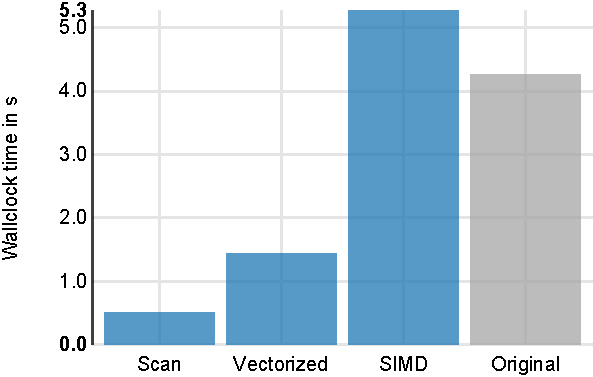
\includegraphics[width=.7\columnwidth]{Figures/damon/SingleThreadedSIMD}
  \caption{SIMD Processing Performance at 50\% Selectivity}
\vspace{-1ex}
  \label{fig:simd-performance}
\end{figure}



\subsubsection*{Multi-threaded}
\label{sec:multi-threaded}
The results of our multi-threaded experiments are displayed in
Figure~\ref{fig:multi-threaded-performance}. To accommodate to the
varying number of cores in our experimentation platforms, we set the
degree of parallelism to the number of (virtual) cores in each machine
(see Table~\ref{tab:hardware}). For reference, we include the best
single-threaded implementation (Vectorized) in the chart. We observe a
significant speedup in almost all cases. Naturally, the \emph{Refined
  Partition \& Merge} implementation performs better than its plain
counterpart. In addition, both implementations achieve a performance
improvement if combined with vectorization. This effect is, however
less pronounced on the highly parallel server systems. On the 96-core
High-End Server system it is virtually non-existent. In general, we
found the \emph{Vectorized Refined Partition \& Merge} implementation
the fastest of our implementation across all parameters. In fact, it
even outperforms (parallel \& predicated) scanning in some cases: the
in-place nature of \emph{Cracking} yields fewer cache-line fill misses
than the out-of-place scan and gives it a (slight) performance edge.


